\documentclass{article}
\setlength{\parskip}{5pt} % esp. entre parrafos
\setlength{\parindent}{0pt} % esp. al inicio de un parrafo
\usepackage{amsmath} % mates
\usepackage[sort&compress,numbers]{natbib} % referencias
\usepackage{url} % que las URLs se vean lindos
\usepackage[top=25mm,left=20mm,right=20mm,bottom=25mm]{geometry} % margenes
\usepackage{hyperref} % ligas de URLs
\usepackage{graphicx} % poner figuras
\usepackage[spanish]{babel} % otros idiomas
\usepackage[utf8]{inputenc}
\author{Elías Alejandro García Bueno \\
Bryan Alejandro Andrade Amaya \\ Jesus Adalberto Mendoza Flores} % author
\title{Tarea 3: El método Monte Carlo} % titulo
\date{15 de septiembre de 2022}

\begin{document} % inicia contenido

\maketitle % cabecera

\begin{abstract} % resumen
Se llama de Montecarlo porque tiene relación con la generación de números aleatorios. Es un método estadístico por el que, a través de números aleatorios, pueden resolverse de manera muy aproximada problemas complejos. Su inventor, en 1947, fue el matemático de origen húngaro, nacionalizado estadounidense, von Newman (1903-1957). Parece ser que la idea le surgió cuando el matemático Stanislaw Ulam (1909-1984) le comentó que había resuelto un complicado solitario, a través de pruebas aleatorias. Von Newman utilizó este método para calcular a qué distancia del suelo debían explotar las bombas de Hiroshima y Nagasaki para que el efecto fuera más devastador.\cite{barreras2015metodo} 

\end{abstract}

\section{Introducción}\label{intro} % seccion y etiqueta
\item 
El termino Monte Carlo se aplica a un conjunto de metodos matemáticos que se empezaron a usar en los 1940s para el desarrollo de armas nucleares en Los Alamos, favorecidos por la aparicion de los ordenadores digitales modernos. Consisten en resolver un problema mediante la invencion de juegos de azar cuyo comportamiento ´ simula algun fenomeno real gobernado por una distribucion de probabilidad (ej. un proceso físico) o sirve para realizar un cálculo (ej. evaluar una integral).
Mas técnicamente, un Monte Carlo es un proceso estocástico numerico, es decir, una ´
secuencia de estados cuya evolucion viene determinada por sucesos aleatorios. Recordemos que un suceso aleatorio es un conjunto de resultados que se producen con cierta probabilidad. \cite{illana2013metodos}


\section{Desarrollo}
\item 
A continuacion se muestra un ejemplo para opbservar como funciona el metodo montecarlo:
\item
Ejemplo 1: Gotas de lluvia para estimar //
Consideremos un circulo de radio unidad circunscrito por un cuadrado. Suponiendo una
lluvia uniforme sobre el cuadrado, podemos hallar el valor de π a partir de la probabilidad de que las gotas caigan dentro del circulo (Figura 1):

\begin{figure} % figura
    \centering
    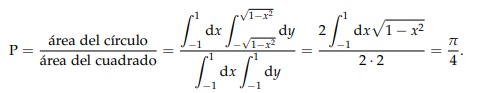
\includegraphics[width=150mm]{Formula.jpg} % archivo
    \caption{Formula del ejemplo}
    \label{formula}
\end{figure}

\item
Es decir, π = 4P. Notese que: (i) podemos simular facilmente este experimento generando aleatoriamente con un ordenador puntos de coordenadas cartesianas (x, y); (ii) podemos mejorar nuestra estimación de π aumentando el numero de puntos generados; (iii) tenemos un metodo para hallar la integral que aparece en la ecuacion (Figura 1). Ciertamente el valor de π puede encontrarse de forma mas rápida y precisa mediante otros metodos, pero veremos que el método Monte Carlo es el más eficiente para hallar integrales multidimensionales (Figura 2).

\begin{figure} % figura
    \centering
    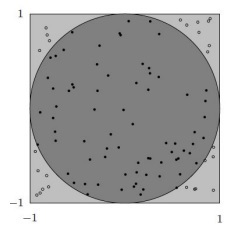
\includegraphics[width=125mm]{Gotas de lluvia.jpg} % archivo
    \caption{Experimento de las gotas de lluvia para estimar π}
    \label{grafica}
\end{figure}

\section{Simulacion}
\item
En en la figura 3 se observa la programacion que se utilizo en el IDE de python para realizar la grafica de montecarlo, y asi mismo se observa en la figura 4 como quedaron los resultados de la grafica.

\begin{figure} % figura
    \centering
    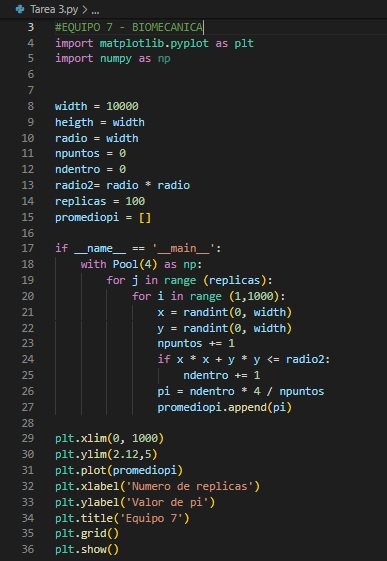
\includegraphics[width=80mm]{Programacion.jpg} % archivo
    \caption{Programacion en python para el metodo monte carlo}
    \label{programa}
\end{figure}

\begin{figure} % figura
    \centering
    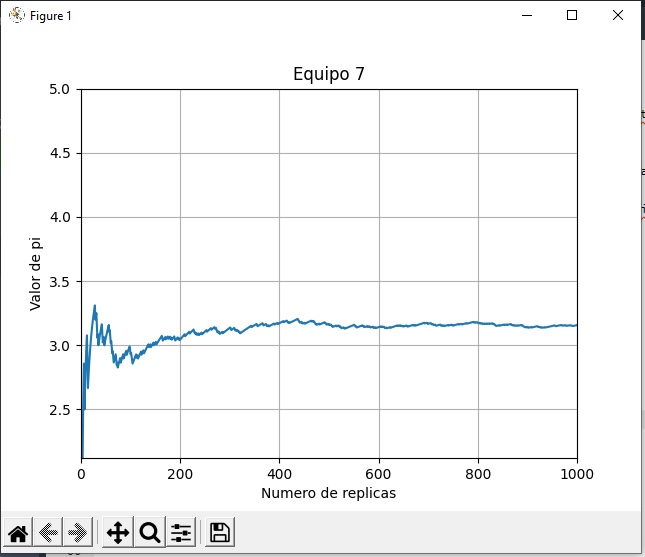
\includegraphics[width=100mm]{Grafica.jpg} % archivo
    \caption{Programacion en python para el metodo monte carlo}
    \label{grafica}
\end{figure}


\section{Conclusiones}
El método de Monte Carlo permite obtener soluciones probabilísticas para ecuaciones donde no es satisfactorio utilizar un método determinístico por falta de precisión en los datos de entrada.
Es muy recomendable hacer uso de un computador para aplicar el método de Monte Carlo. Éste puede realizar las cientos o miles de simulaciones necesarias en pocos segundos y con la cantidad de cifras decimales necesarias.
Ahora que conocemos este metodo sera de gran utilidad para aplicarlo cuando se este realizando algun trabajo o proyecto de otra materia, asi como tambien lo podemos aplicar en nuestra vida laboral ya que es de gran utilizad.


\bibliographystyle{plainnat}
\bibliography{bibliografia.bib}



\end{document}